\documentclass[12pt, a4paper]{article}
\usepackage{graphicx}
\usepackage{xcolor}
\renewcommand{\contentsname}{Inhaltsverzeichnis}
\renewcommand{\figurename}{Abb.}
\newcommand\crule[3][black]{\textcolor{#1}{\rule{#2}{#3}}}
\definecolor{yellow570}{RGB}{237, 255, 0}
\definecolor{green550}{RGB}{0, 255, 0}
\definecolor{orange590}{RGB}{255, 171, 0}
\definecolor{cyan490}{RGB}{0, 194, 222}
\definecolor{green510}{RGB}{0, 250, 92}
\definecolor{green500}{RGB}{0, 236, 168}

\begin{document}
\begin{titlepage}
\begin{center}
    \LARGE{Spektroskopie} \\
    \large{Protokoll} \\
    \vspace{10mm}
    
\includegraphics[width=\textwidth]{Spektrum.png} \\
    \vspace{10mm}
    \small{Ort} \\
    \Large{ BBS Papenburg,\\ 
            Raum B007a} \\
    \vspace{10mm}
    \small{Zeitraum} \\
    \Large{ 06.02.2020 \\
            13:45 - 15:15} \\
    \vspace{15mm}
    \small{Protokollanten} \\
    \Large{ Connor Kr\"oger,\\
            Mathis Mensing,\\
            Jana Schwarz}
\end{center}

\thispagestyle{empty}
\end{titlepage}

\tableofcontents
\newpage

\section{Ziel des Experiments}
Das Ziel des Experiments ist das Darstellen des Spektrums einer polychromatischen Lichtquelle.

\section{Versuchsaufbau}
\subsection{Materialien}

\begin{itemize}
    \item geradlinige Schiene
    \item 6 Stativhalterungen, passend zur Schiene
    \item Gleichspannungsnetzteil zum Betreiben der Lichtquelle
\end{itemize}
\begin{enumerate}
    \item polychromatische (nat\"urliche) Lichtquelle in Form einer Halogenbirne (12V, max. 10W)
    \item Schirm zur Abschirmung des Raumes von Streulicht
    \item Fokallinse mit 50mm Brennweite
    \item Kollimator (Parallelisierungslinse) mit 100mm Brennweite
    \item verschiedene Farbfilter
    \item einstellbarer Spalt
    \item optisches Gitter
    \item Projektionsschirm (in diesem Fall eine weiße Wand)
\end{enumerate}
\newpage

\subsection{Aufbau}
\begin{figure}[h]
    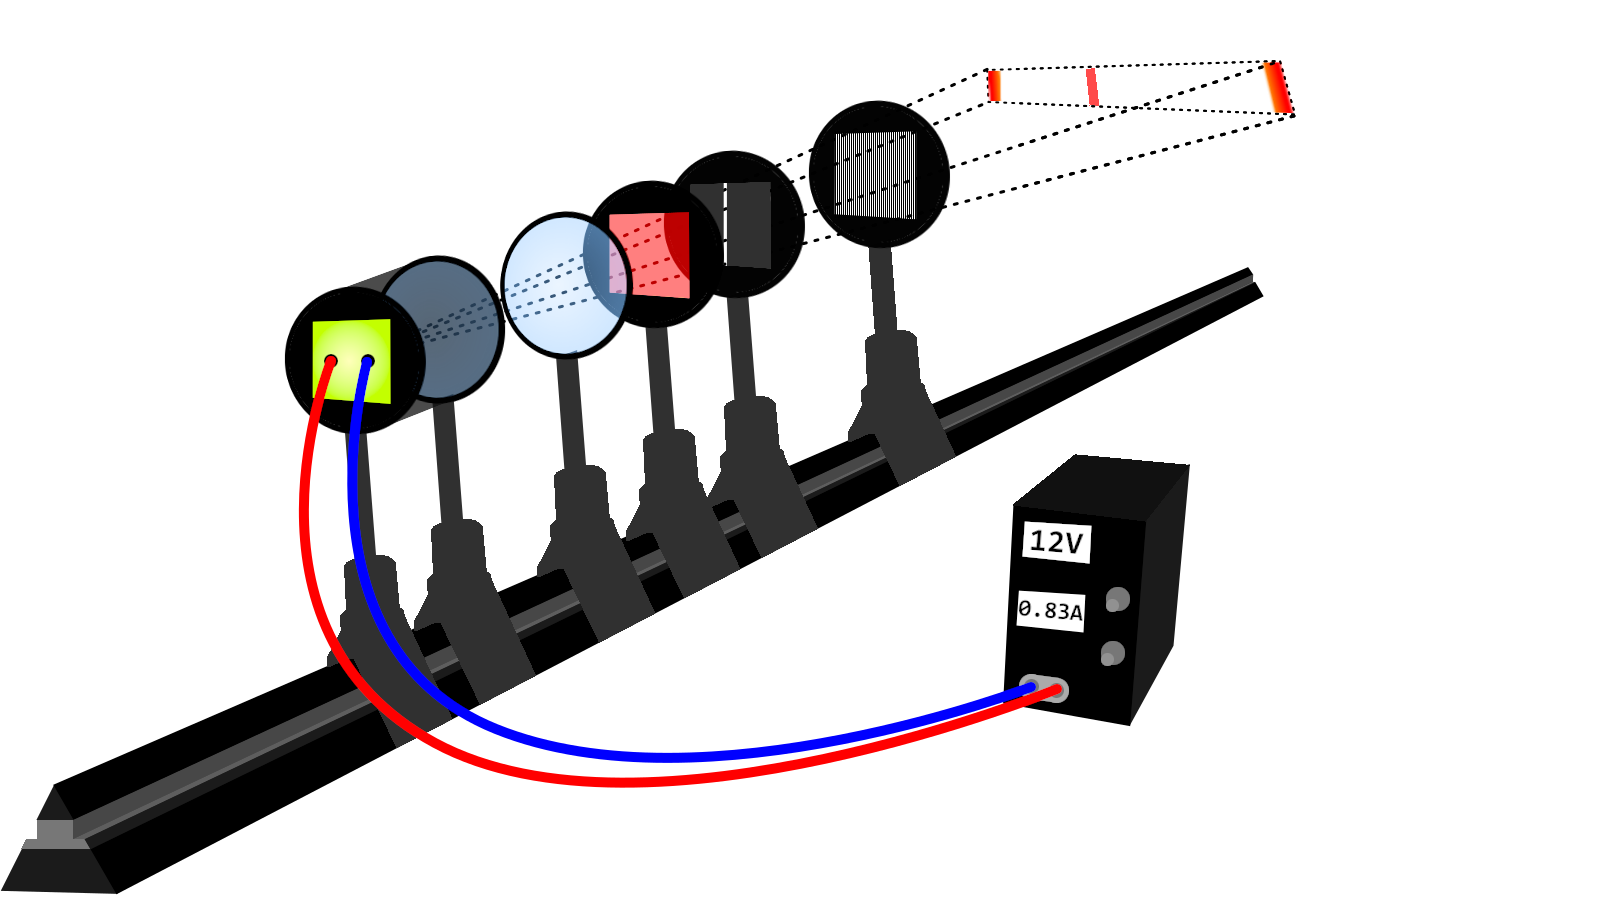
\includegraphics[width=\textwidth]{Aufbau.png}
    \caption[Aufbau]{Aufbau des Experiments}
\end{figure}

Das Gleichspannungsnetzteil wird an die Halogenbirne angeschlossen.
Die verschiedenen Elemente werden in o.g. Reihenfolge in Stative auf einer geraden Schiene verbaut.
Wichtig ist hierbei, dass Lichtquelle, Linsen, Filter, Spalt und Gitter auf einer Sichtlinie stehen,
sodass das Licht weder ungewollt abgelenkt wird noch verloren geht. Der Schirm wird \"uber der Lichtquelle und der Fokallinse angebracht,
sodass Streulicht den Raum nicht erhellt und somit ein erh\"ohter Kontrast erzielt wird. Die Fokallinse wird in einem Abstand von ca.
5cm zur Lichtquelle angebracht; die Parallelisierungslinse ca. 10cm von der Fokallinse; der Farbfilter in einem beliebigem Abstand
zum Kollimator (sodass das gesamte emittierte Licht erfasst wird); der einstellbare Spalt so, dass er vom gesamten Licht erfasst wird;
das optische Gitter so, dass es vertikal vom gesamten Lichtspalt erfasst wird.\\Eventuell m\"ussen die Abst\"ande durch Probieren so angepasst werden, dass ein scharfes Spektrum erzeugt wird. Die genannten Werte dienen zur Orientierung.

\newpage
\section{Durchf\"uhrung}
Das Gleichspannungsnetzteil wird auf eine Spannung von 12V eingestellt, sodass die Halogenbirne Licht emittiert.
Der gesamte Versuch wird auf einer Schiene in Richtung zur Wand positioniert. Werden die Fokallinse in einem Abstand von 5cm von der
Lampe und die Parallelisierungslinse im Abstand von 10cm von der Fokallinse richtig angebracht, und ist die Gl\"uhlampe am Leuchten, sollte an der Wand ein deutlich zu erkennender Lichtfleck zu sehen sein.
Ist dieser verschwommen, kann es sein, dass das Licht ungewollt abgelenkt wird. In diesem Fall m\"ussen die Abst\"ande der Linsen zueinander und zu der Gl\"uhlampe ver\"andert werden,
bis das an der Wand abgebildete Licht klar zu erkennen ist. So f\"ahrt man ebenfalls mit dem einstellbaren Spalt und dem optischen Gitter fort.
Diese werden so angebracht, dass sie vom ganzen Licht erfasst werden. Sieht man an die Wand, erkennt man, dass nun nicht mehr nur ein Lichtfleck zu sehen ist,
sondern auch Spektralfarben, die sich beidseitig in einem Abstand von der Mitte befinden. Man kann hier ebenfalls durch Verschieben der Linsen die Genauigkeit der Farben einstellen.
Bei diesem Versuch sollte der Raum m\"oglichst dunkel sein, um die Farben klar erkennen zu k\"onnen.\\Durch sogenannte Farbfilter kann man im Anschluss bestimmte Wellenl\"angen herausfiltern, sodass beispielsweise nur die Farbe Rot zu sehen ist.

\section{Auswertung}
Das polychromatische Licht wird durch das optische Gitter in seine einzelnen Wellenl\"angen aufgeteilt und gebrochen, sodass, mit der Annahme, dass kein Farbfilter installiert ist,
auf dem Projektionsschirm mittig ein weißer Strich und jeweils außen die Spektren entstehen.
Anhand der Spektren kann man erkennen, aus welchen Wellenl\"angen das Licht besteht bzw.
welche Wellenl\"angen der jeweilige Farbfilter durchl\"asst - darauß l\"asst sich u.A. z.B. die Qualit\"at des Farbfilters bestimmen.

\begin{figure}[h]
    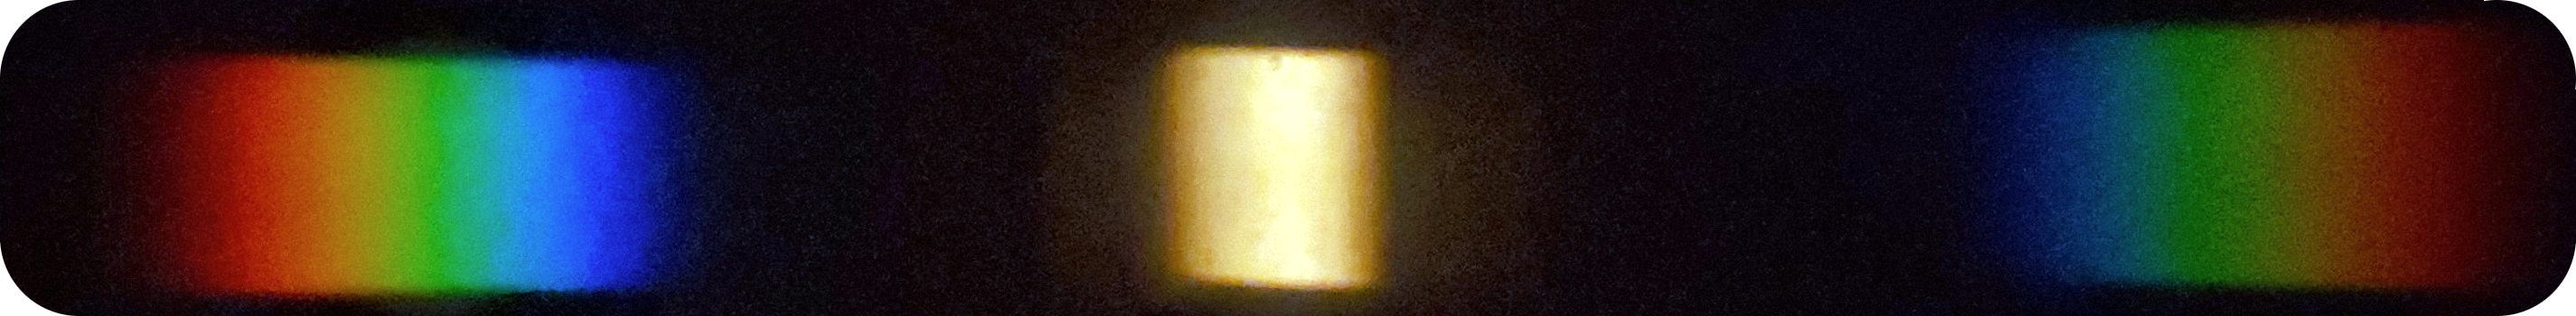
\includegraphics[width=\textwidth]{Spektrum_Foto.png}
    \caption[Ergebnis]{Ergebnis des Experiments}
\end{figure}

\section{G\"ute eines optischen Filters}
Optische Filter haben eine sogenannte G\"ute, die angibt, wie Farbtreu diese sind.
Die Güte wird, genau wie die Farbe bzw. Wellenl\"ange des Lichts selbst, in $nm$ angegeben.
Somit l\"asst ein Farbfilter mit der Wellenl\"ange $570nm$ (\crule[yellow570]{3mm}{3mm} gelb) mit einer Güte von $\pm 20nm$ Licht im Bereich
von $550nm$ (\crule[green550]{3mm}{3mm} gr\"un) bis $590nm$ (\crule[orange590]{3mm}{3mm} orange) durch.\\
\\
Dasselbe l\"asst sich auch in umgekehrter Richtung durchf\"uhren; man kann also aus dem erschienenen
Spektrum die Wellenl\"ange und G\"ute des Filters errechnen.
Hat man beispielsweise ein Spektrum, welches bei $490nm$ (\crule[cyan490]{3mm}{3mm} cyan) anf\"angt und bei $510nm$ (\crule[green510]{3mm}{3mm} gr\"un) endet,
errechnet man aus den beiden Werten zun\"achst den Mittelwert $\bar\lambda=\frac{\lambda_1+\lambda_2}{2}=\frac{490nm + 510nm}{2}=500nm$ (\crule[green500]{3mm}{3mm} gr\"un).
Die G\"ute l\"asst sich dann durch $\bar\lambda - \lambda_1 = 500nm - 490nm = 10nm$ errechnen.
Der Filter hat also eine Wellenl\"ange von $500nm$ mit einer Güte von $\pm 10nm$.\\
Den Bereich des Spektrums kann man in diesem Fall entweder sch\"atzen oder mittels linearer Zuordnung errechnen. Für letzteres ben\"otigt man allerdings
bereits mindestens zwei Punkte im Spektrum, dessen Wellenl\"ange bekannt ist.

\end{document}
